\documentclass[11pt]{article}

\usepackage[a4paper,margin=1in]{geometry}
\usepackage{amsmath,amssymb,mathtools}
\usepackage{booktabs}
\usepackage{graphicx}
\usepackage{microtype}
\usepackage{caption}
\usepackage{float}
\usepackage{xcolor}
\usepackage{enumitem}
\usepackage{hyperref}

\graphicspath{{../results/figures/}}
\hypersetup{
  colorlinks=true,
  linkcolor=blue!45!black,
  citecolor=blue!45!black,
  urlcolor=blue!45!black,
  pdftitle={Bayesian Learning and Model Risk in a Binary Market-Making Model},
  pdfauthor={Mohamed Rayan Bouchaibi}
}

\newcommand{\SpreadMaxError}{0.087}
\newcommand{\RmseDropAtTwenty}{40.7\%}
\newcommand{\PnlSdDropAtTwenty}{61.1\%}
\newcommand{\MedianHitTwenty}{28}
\newcommand{\MedianHitForty}{8}
\newcommand{\PairedRmseDeltaTwenty}{-4.07}
\newcommand{\PairedRmseCiLow}{-4.15}
\newcommand{\PairedRmseCiHigh}{-3.99}
\newcommand{\MisspecPnl}{-19.09}
\newcommand{\CorrectPnl}{0.41}
\newcommand{\MisspecRmse}{3.61}
\newcommand{\CorrectRmse}{3.13}
\newcommand{\JointAlphaMae}{0.067}
\newcommand{\RollingReachRate}{99.1\%}
\newcommand{\RollingMedianDelay}{17}
\newcommand{\RollingPostMae}{0.117}
\newcommand{\FullHistoryReachRate}{13.0\%}
\newcommand{\FullHistoryPostMae}{0.235}
\newcommand{\InventoryExposureDrop}{56.8\%}
\newcommand{\InventoryRiskDrop}{68.3\%}
\newcommand{\InventoryMeanPnlDrop}{3.9\%}
\newcommand{\BestHalfSpread}{1.00}
\newcommand{\BestHalfSpreadPnl}{78.61}
\newcommand{\BestHalfSpreadFills}{81.5}
\newcommand{\ResultsEngine}{ocaml}
\newcommand{\ResultsProfile}{full}
\newcommand{\ResultsSeed}{20260831}

\newcommand{\StrategyRows}{%
0.05 & 10.00 & 9.46 & 78.04 & 71.12 \\
0.20 & 10.00 & 5.84 & 76.36 & 29.00 \\
0.40 & 10.00 & 3.15 & 70.75 & 12.33 \\
}

\newcommand{\RegimeRows}{%
full history & 12.1\% & 64 & 0.236 \\
rolling 20 & 99.5\% & 17 & 0.117 \\
rolling 50 & 94.4\% & 40 & 0.126 \\
rolling 100 & 81.8\% & 68 & 0.178 \\
}


\title{Bayesian Learning and Model Risk in a Binary Market-Making Model\\
\large A Reproducible Computational Note on Adverse Selection, Misspecification, and Regime Change}
\author{Mohamed Rayan Bouchaibi\\
\small Mathematics Section, School of Basic Sciences\\
\small \'Ecole polytechnique f\'ed\'erale de Lausanne (EPFL), Lausanne, Switzerland}
\date{September 2026}

\begin{document}
\maketitle

\begin{center}
\small Independent technical report. Not peer reviewed.\\
\small This work was conducted independently and is not an official publication or endorsement of EPFL.
\end{center}

\begin{abstract}
This note studies a small market-making model in which a terminal asset value is binary and incoming traders are either informed or liquidity-motivated. The model is intentionally restrictive because it admits analytical benchmarks that can be used to audit the simulator. Competitive bid and ask prices are derived for a general prior, sequential learning is expressed in log-odds form, and the information rate of order flow is made explicit. An OCaml implementation is then used to examine static and Bayesian quoting, misspecification of the informed-trader probability, joint inference of value and information intensity, and adaptation after an abrupt regime change. A separate quote-sensitive execution model is retained as an appendix to show why inventory claims require price-dependent fills. The simulations reproduce the analytical spread to within \SpreadMaxError\ price units over the tested grid. At $\alpha=0.20$, Bayesian updating reduces fair-value root mean squared error by \RmseDropAtTwenty\ and terminal P\&L standard deviation by \PnlSdDropAtTwenty\ relative to a static belief. The main contribution is methodological: analytical identities, hidden-state boundaries, paired random worlds, independent implementations, and explicit failure modes make the numerical claims auditable. The results describe the stated models and do not constitute evidence of live-market profitability.
\end{abstract}

\noindent\textbf{Keywords:} Bayesian inference; market microstructure; market making; adverse selection; model misspecification; sequential learning; regime change.

\section{Introduction}

A market maker posts prices before knowing why the next customer will trade. A buy can represent ordinary demand for immediacy, or it can come from a trader who knows that the asset is worth more than the posted ask. The execution is therefore both a transaction and an observation about the hidden value.

Glosten and Milgrom formalised this mechanism in a sequential dealer market where adverse selection generates a positive spread even for a risk-neutral specialist earning zero expected profit \cite{glosten_milgrom_1985}. This note uses a deliberately smaller version of that information structure. The objective is not to approximate a modern electronic limit order book. The objective is to build a model whose quotes, posterior updates, and accounting can be derived independently of the code, then use that benchmark to study what happens when the information parameter is wrong, unknown, or unstable.

The central question is:

\begin{quote}
How should a competitive market maker update prices when order direction is informative, and which numerical conclusions remain defensible when the information environment is misspecified or non-stationary?
\end{quote}

The contribution is a reproducible computational note rather than a new equilibrium model. Three features are emphasised. First, the competitive spread is derived for a general prior, not only for the symmetric starting point. Second, the log-odds dynamics expose the information rate of order flow and explain why a larger informed fraction simultaneously increases adverse-selection risk and accelerates learning. Third, the simulation is treated as an object to audit. Hidden state is isolated from the strategy interface, competing strategies see identical order tapes, a separate NumPy implementation repeats the equations, and output-level checks reject several classes of attractive but invalid result.

\section{Related Work and Positioning}

The information model is a simplified descendant of Glosten and Milgrom \cite{glosten_milgrom_1985}; standard market microstructure treatments place the model within the broader distinction between inventory, information, and strategic-trading explanations of spreads \cite{ohara_1995}. Das studies a learning market maker in an extension of the Glosten-Milgrom setting with noisy signals and a changing fundamental value \cite{das_2005}. The present note is narrower in market structure but focuses explicitly on analytical test oracles, misspecification of the informed fraction, joint parameter inference, and reproducible numerical provenance.

The inventory appendix is conceptually separate. Its quote-sensitive fill mechanism is motivated by the inventory and execution trade-off studied by Avellaneda and Stoikov \cite{avellaneda_stoikov_2008} and by Gu\'eant, Lehalle, and Fernandez-Tapia \cite{gueant_2013}. The linear inventory skew used here is not an optimal-control solution. It is retained only to show how a price-dependent arrival mechanism changes what can be inferred from simulated P\&L.

The regime-change experiment uses a rolling window as a transparent heuristic. A principled extension would replace it with a latent-state or online changepoint model, such as Bayesian online changepoint detection \cite{adams_mackay_2007}.

\section{Binary Information Model}

\subsection{Terminal value and order flow}

The terminal value is
\begin{equation}
V\in\{L,H\}, \qquad L<H,
\end{equation}
with prior
\begin{equation}
P(V=H)=p.
\end{equation}
The baseline parameters are
\begin{equation}
L=90, \qquad H=110, \qquad p_0=\frac{1}{2}.
\end{equation}

Each arriving trader is informed with probability $\alpha$. An informed trader observes $V$ perfectly and buys in the high state or sells in the low state. A noise trader buys or sells with equal probability. Therefore
\begin{align}
P(Buy\mid H)&=\frac{1+\alpha}{2},\\
P(Buy\mid L)&=\frac{1-\alpha}{2}.
\end{align}
The sell probabilities follow by symmetry.

This is a deliberately severe abstraction. Real information is noisy, trade sizes vary, traders may split orders strategically, and observed order flow is affected by prices, latency, venue choice, and competition. The binary construction is useful because the inference mechanism remains visible.

\subsection{Competitive quotes for a general prior}

Let $p_t=P(V=H\mid\mathcal{F}_t)$ be the market maker's belief before the next trade. A competitive risk-neutral ask and bid are conditional expectations:
\begin{align}
A_t&=E[V\mid Buy,\mathcal{F}_t],\\
B_t&=E[V\mid Sell,\mathcal{F}_t].
\end{align}

Bayes' rule gives
\begin{align}
P(H\mid Buy,\mathcal{F}_t)
&=\frac{p_t(1+\alpha)}{1+\alpha(2p_t-1)},\\
P(H\mid Sell,\mathcal{F}_t)
&=\frac{p_t(1-\alpha)}{1-\alpha(2p_t-1)}.
\end{align}
Hence
\begin{align}
A_t
&=L+(H-L)\frac{p_t(1+\alpha)}{1+\alpha(2p_t-1)},\\
B_t
&=L+(H-L)\frac{p_t(1-\alpha)}{1-\alpha(2p_t-1)}.
\end{align}
Subtracting the two expressions gives
\begin{equation}
\boxed{
A_t-B_t
=(H-L)\frac{4\alpha p_t(1-p_t)}{1-\alpha^2(2p_t-1)^2}
}.
\end{equation}

At the symmetric prior $p_t=1/2$,
\begin{equation}
\boxed{A_t-B_t=(H-L)\alpha.}
\end{equation}
For $L=90$, $H=110$, and $\alpha=0.20$, the initial quote is $98/102$.

The general formula adds an important interpretation. As the posterior approaches either zero or one, value uncertainty disappears and the informational spread converges toward zero. The symmetric-prior formula is therefore the widest point for a fixed $\alpha$ in this binary setting, not a spread that remains constant throughout learning.

\subsection{Sequential learning and information rate}

After a buy,
\begin{equation}
p_{t+1}
=\frac{p_tP(Buy\mid H)}{p_tP(Buy\mid H)+(1-p_t)P(Buy\mid L)},
\end{equation}
and the sell update is analogous. Define log odds
\begin{equation}
\ell_t=\log\frac{p_t}{1-p_t}
\end{equation}
and the per-trade evidence magnitude
\begin{equation}
\lambda(\alpha)=\log\frac{1+\alpha}{1-\alpha}.
\end{equation}
Then
\begin{equation}
\ell_t
=\ell_0+(N_B-N_S)\lambda(\alpha),
\end{equation}
where $N_B$ and $N_S$ are cumulative buys and sells.

Under the high state, a buy occurs with probability $(1+\alpha)/2$ and a sell with probability $(1-\alpha)/2$. Therefore
\begin{equation}
E[\ell_{t+1}-\ell_t\mid H]
=\alpha\lambda(\alpha).
\end{equation}
Under the low state the drift is the negative of the same quantity. This quantity is also the Kullback-Leibler divergence between the order-side distributions under the two states. A larger $\alpha$ therefore has two effects inside the same model: it widens the adverse-selection spread and increases the expected rate at which order flow reveals the hidden state.

\subsection{Conditional zero profit under correct competitive quoting}

The competitive quote has a useful accounting identity. Conditional on a customer buy,
\begin{equation}
E[A_t-V\mid Buy,\mathcal{F}_t]=0,
\end{equation}
because $A_t=E[V\mid Buy,\mathcal{F}_t]$. Similarly,
\begin{equation}
E[V-B_t\mid Sell,\mathcal{F}_t]=0.
\end{equation}
Thus a correctly specified competitive Bayesian market maker has zero expected economic P\&L on each trade conditional on the information available when the quote is formed. Simulation should not be expected to discover positive expected profit in that model. The relevant comparisons are estimation error, risk concentration, and the consequences of misspecification.

\subsection{A one-trade benchmark for misspecification}

The execution assumption makes the sign of misspecification P\&L analytically visible before any sequential learning occurs. Suppose the true informed fraction is $\alpha$, the market maker uses $\widehat{\alpha}$, and the state prior $p$ itself is correct. If every arriving order executes, the expected market-maker P\&L on the next trade is
\begin{equation}
E[\Pi_1]
=(H-L)\frac{2p(1-p)(\widehat{\alpha}-\alpha)}{1-\widehat{\alpha}^{2}(2p-1)^2}.
\end{equation}
At the symmetric prior,
\begin{equation}
\boxed{
E[\Pi_1]=\frac{H-L}{2}(\widehat{\alpha}-\alpha)
}.
\end{equation}
Underestimating information intensity therefore creates a negative expected one-trade P\&L, while overestimating it creates a positive expected value in this forced-execution environment. The positive side is not evidence that overly wide quotes are economically optimal. It follows directly from charging a larger adverse-selection premium without losing order flow. This identity is a useful benchmark for interpreting the later misspecification surface.

\subsection{Cash, inventory, and terminal wealth}

Trade direction is defined from the customer's perspective. A customer buy means the market maker sells one unit at the ask:
\begin{align}
C_{t+1}&=C_t+A_t,\\
q_{t+1}&=q_t-1.
\end{align}
A customer sell means the market maker buys at the bid:
\begin{align}
C_{t+1}&=C_t-B_t,\\
q_{t+1}&=q_t+1.
\end{align}
Terminal wealth is
\begin{equation}
W_T=C_T+q_TV.
\end{equation}
The simulator also records trade-level economic P\&L. Selling at the ask contributes $A_t-V$, while buying at the bid contributes $V-B_t$. Automated tests reconcile the sum of these quantities with terminal cash plus marked inventory.

\section{Unknown and Changing Information Intensity}

When $\alpha$ is unknown, the market maker places prior mass on a finite candidate grid and maintains
\begin{equation}
P(V,\alpha\mid\mathcal{F}_t).
\end{equation}
For an observed side $D_t\in\{Buy,Sell\}$,
\begin{equation}
P(V,\alpha\mid\mathcal{F}_t)
\propto
P(D_t\mid V,\alpha)P(V,\alpha\mid\mathcal{F}_{t-1}).
\end{equation}
Quotes integrate over both sources of uncertainty.

This model has an identification problem. A run of buys can be explained by a high terminal value, a large informed fraction, or both. One short tape with one fixed hidden value does not cleanly separate those explanations. The joint filter is therefore evaluated as an estimator with visible uncertainty, not treated as a strictly superior replacement for a correctly specified fixed-parameter model.

The stationary assumption is then violated deliberately. The simulation changes $\alpha$ from $0.05$ to $0.40$ halfway through an episode. A full-history filter remains Bayesian under the wrong assumption that one constant $\alpha$ generated the complete tape. Rolling filters rebuild the joint posterior from only the most recent $w$ observations. They adapt faster by discarding evidence, which increases variance and introduces a tuning parameter.

\section{Experimental Design}

\subsection{Evaluation questions}

The numerical experiments evaluate eight claims:
\begin{enumerate}[label=Q\arabic*.]
\item Does the simulated conditional-value spread recover the analytical benchmark?
\item Does larger $\alpha$ produce faster posterior concentration, as implied by the log-odds drift?
\item How much do sequential Bayesian beliefs change fair-value error and P\&L dispersion relative to a frozen belief?
\item What are the consequences of underestimating or overestimating $\alpha$?
\item How accurately can a finite-grid joint posterior separate value from information intensity?
\item How does a full-history filter behave after the stationarity assumption fails, compared with finite-memory estimators?
\item In a separate quote-sensitive execution model, how does inventory skew alter position exposure and P\&L dispersion?
\item Once fill probability responds to quote distance, does the tested spread grid produce an interior profit maximum?
\end{enumerate}

\subsection{Monte Carlo protocol}

The full run uses seed \ResultsSeed. Spread validation contains 100,000 one-trade trials per value of $\alpha$. Price discovery uses 3,000 paths of 80 trades. Static-versus-Bayesian comparison uses 6,000 episodes of 60 trades at each information level. The misspecification grid uses 1,800 episodes for every $(\alpha,\widehat{\alpha})$ pair, and the unknown-$\alpha$ study uses 2,500 episodes of 80 trades. The regime experiment uses 800 paths of 200 trades, switching after trade 100. The inventory appendix uses 3,500 paths of 300 steps.

Competing strategies face identical hidden states and order tapes. Inventory policies reuse episode-indexed random streams across parameter values. Common random numbers do not change expectations, but they reduce Monte Carlo noise in paired differences.

The principal information-model metrics are terminal P\&L, P\&L standard deviation, fifth percentile, fair-value RMSE, informed-flow P\&L, noise-flow P\&L, quoted spread, posterior confidence, and threshold hitting times. The regime estimator is considered adapted when its $\alpha$ estimate lies within $0.10$ of the new value for five consecutive observations.

The reported confidence intervals quantify Monte Carlo uncertainty in simulation averages. They are not empirical confidence intervals for market behaviour.

\section{Results}

\subsection{Analytical spread validation}

Figure~\ref{fig:spread} compares the closed-form symmetric-prior spread with its Monte Carlo conditional-value estimate. The largest absolute discrepancy over the tested grid is \SpreadMaxError\ price units.

\begin{figure}[H]
\centering
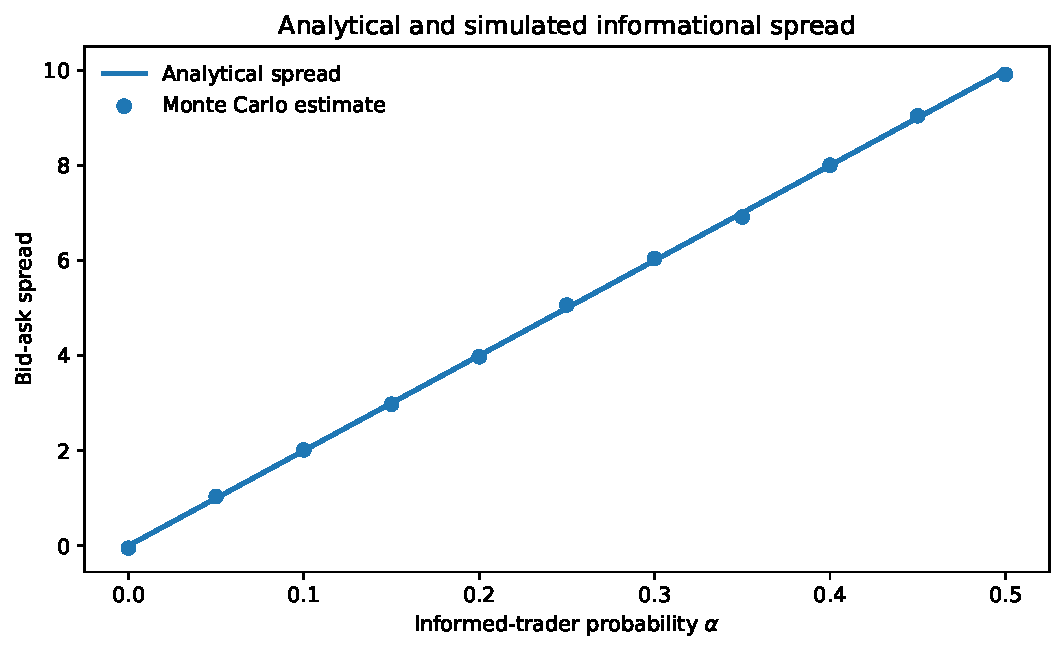
\includegraphics[width=0.82\textwidth]{01_spread_validation.pdf}
\caption{Theoretical and simulated informational spread at the symmetric prior.}
\label{fig:spread}
\end{figure}

This is an implementation check rather than an empirical result. A material failure here would invalidate the later numerical comparisons.

\subsection{Price discovery}

Figure~\ref{fig:discovery} shows posterior confidence assigned to the true state. Posterior odds move on a discrete lattice determined by net order imbalance, so median trajectories can be jagged even when the expected direction is monotone.

\begin{figure}[H]
\centering
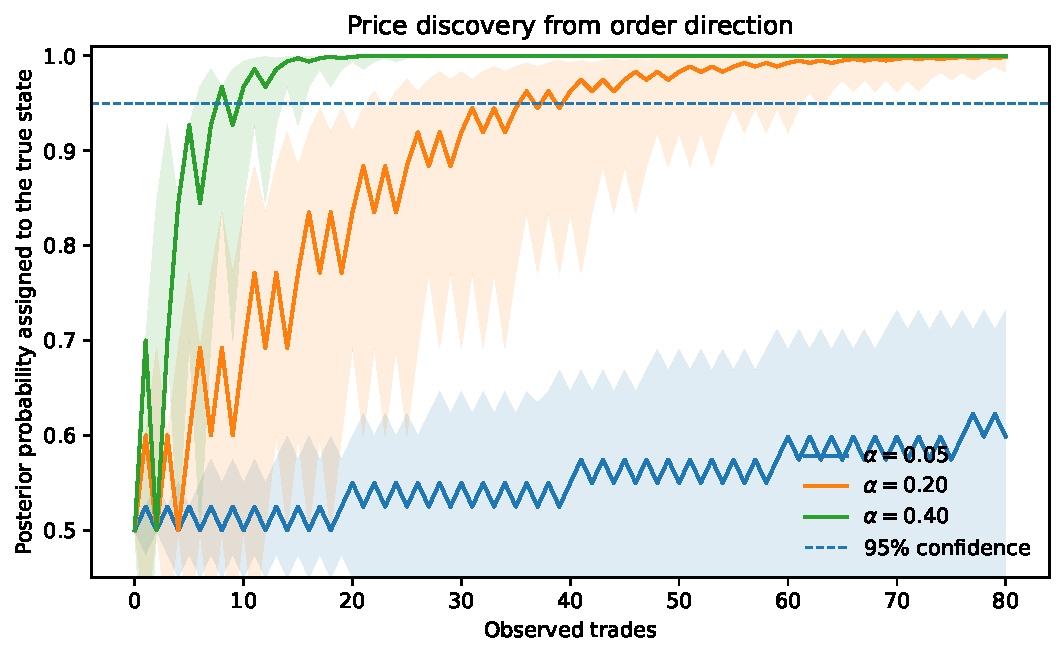
\includegraphics[width=0.86\textwidth]{02_price_discovery.pdf}
\caption{Median posterior confidence, with interquartile bands.}
\label{fig:discovery}
\end{figure}

At $\alpha=0.20$, paths that reach 95\% confidence do so after a median of \MedianHitTwenty\ trades. At $\alpha=0.40$, the corresponding median is \MedianHitForty\ trades. The analytical log-odds drift explains the direction of this effect: more informative flow is more dangerous before it is learned from, but also more revealing.

\subsection{Static and Bayesian beliefs}

The static strategy holds $p_t=0.5$ throughout the episode. The Bayesian strategy updates after every observed order side. Table~\ref{tab:strategy} reports selected results.

\begin{table}[H]
\centering
\caption{Estimation error and P\&L dispersion under static and Bayesian beliefs.}
\label{tab:strategy}
\begin{tabular}{ccccc}
\toprule
$\alpha$ & Static RMSE & Bayesian RMSE & Static P\&L SD & Bayesian P\&L SD \\
\midrule
\StrategyRows
\bottomrule
\end{tabular}
\end{table}

At $\alpha=0.20$, Bayesian updating lowers RMSE by \RmseDropAtTwenty\ and P\&L standard deviation by \PnlSdDropAtTwenty. Mean profit remains close to zero, which is the expected benchmark for correctly specified competitive quotes.

\begin{figure}[H]
\centering
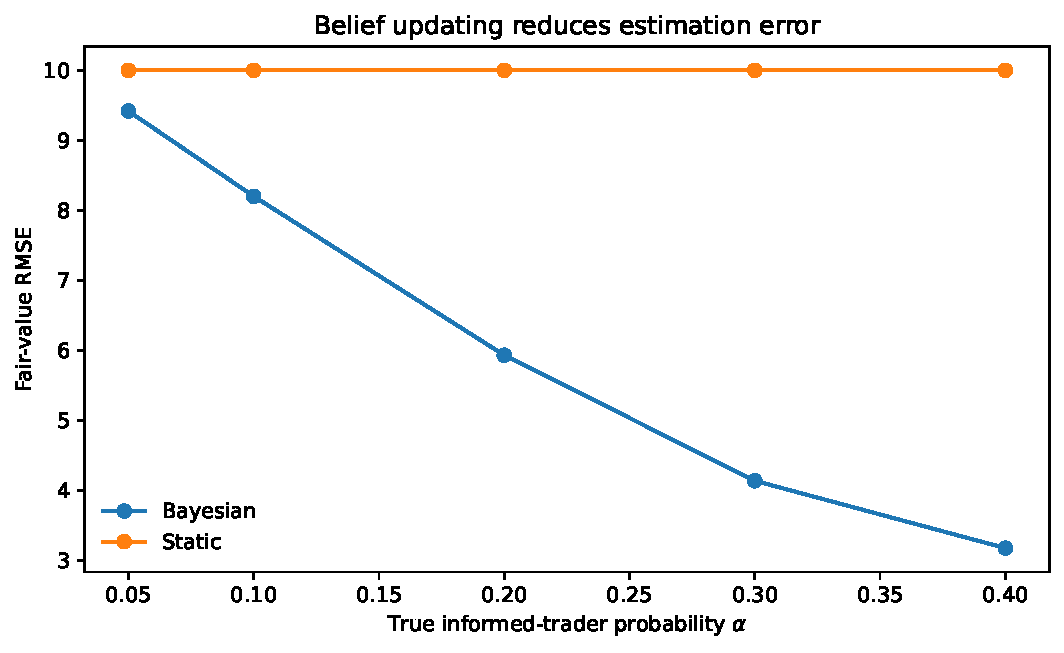
\includegraphics[width=0.78\textwidth]{03_strategy_rmse.pdf}
\caption{Fair-value RMSE under static and Bayesian beliefs.}
\label{fig:rmse}
\end{figure}

\begin{figure}[H]
\centering
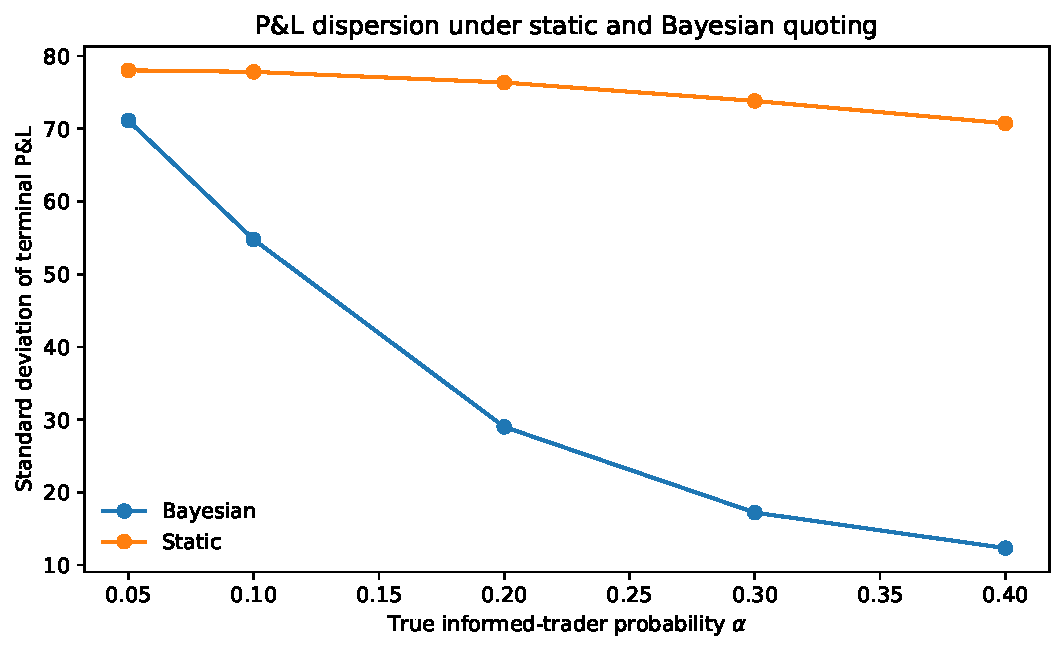
\includegraphics[width=0.78\textwidth]{04_strategy_pnl_dispersion.pdf}
\caption{Terminal P\&L dispersion under static and Bayesian beliefs.}
\label{fig:pnl-dispersion}
\end{figure}

Because both strategies see the same simulated episodes, the episode-level difference can be measured directly. At $\alpha=0.20$, the mean Bayesian-minus-static RMSE difference is \PairedRmseDeltaTwenty, with an approximate 95\% Monte Carlo interval of $[\PairedRmseCiLow,\PairedRmseCiHigh]$.

\begin{figure}[H]
\centering
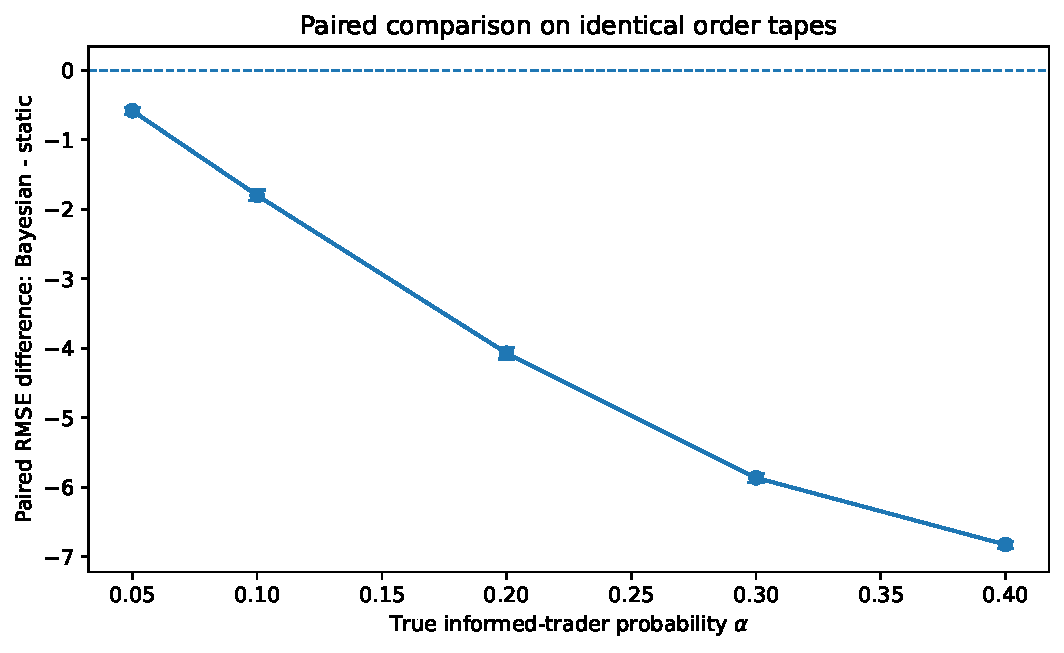
\includegraphics[width=0.78\textwidth]{05_paired_rmse_difference.pdf}
\caption{Paired RMSE differences on identical order tapes. Bars show approximate 95\% Monte Carlo intervals for the mean difference.}
\label{fig:paired-rmse}
\end{figure}

The static strategy's RMSE is exactly 10 in the baseline because it always values the asset at 100 while the realised terminal value is 90 or 110. The size of the RMSE reduction is therefore a structural property of this toy problem and should be read as a validation result, not as evidence of an economic edge.

\subsection{Misspecifying the informed fraction}

The misspecification experiment separates the true $\alpha$ from the market maker's assumed value $\widehat{\alpha}$.

\begin{figure}[H]
\centering
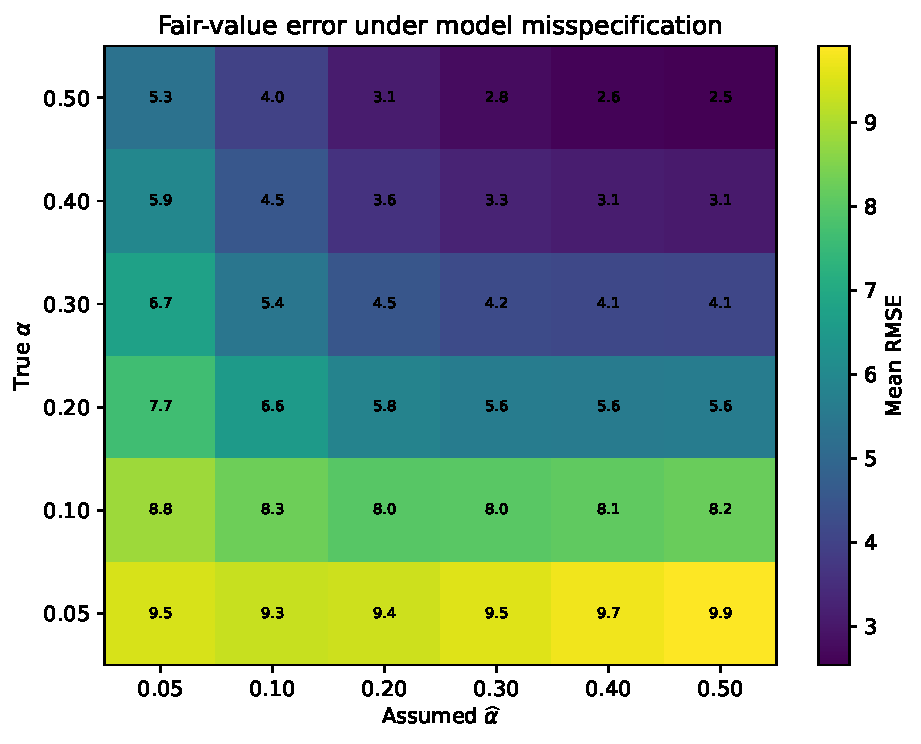
\includegraphics[width=0.76\textwidth]{06_misspecification_rmse.pdf}
\caption{Fair-value RMSE under misspecification.}
\label{fig:misspec-rmse}
\end{figure}

\begin{figure}[H]
\centering
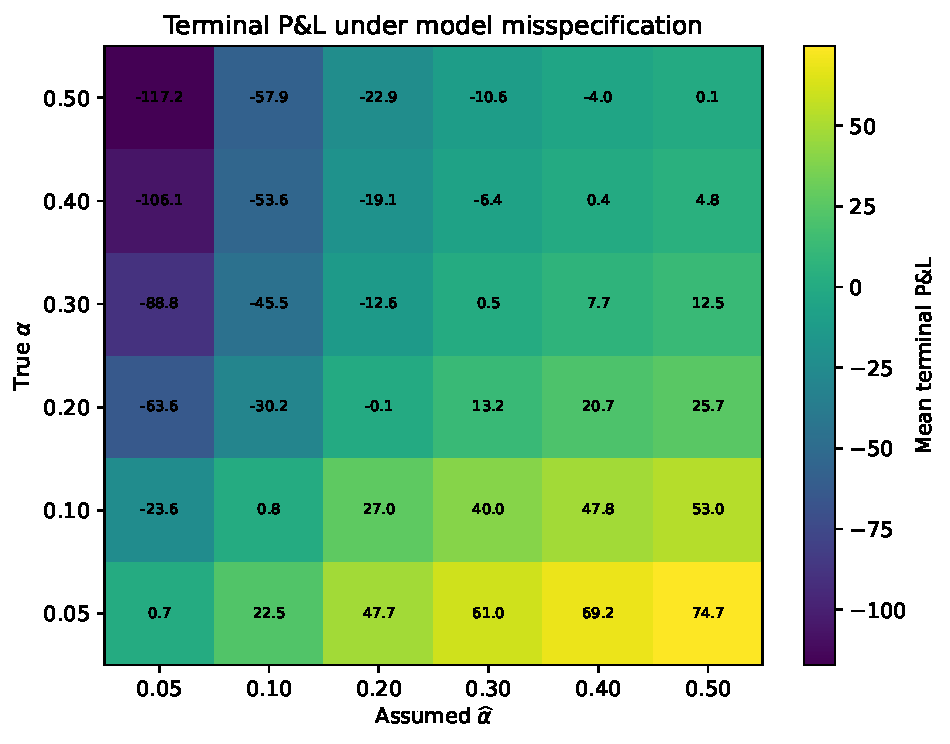
\includegraphics[width=0.76\textwidth]{07_misspecification_pnl.pdf}
\caption{Mean terminal P\&L under misspecification.}
\label{fig:misspec-pnl}
\end{figure}

When the true value is $\alpha=0.40$ but the strategy assumes $0.20$, mean terminal P\&L is \MisspecPnl\ and fair-value RMSE is \MisspecRmse. Under correct specification, the corresponding values are \CorrectPnl\ and \CorrectRmse. Underestimation leaves quotes too tight for the information content of the incoming flow.

Overestimation often produces positive mean P\&L in Figure~\ref{fig:misspec-pnl}. The one-trade benchmark shows that the sign is already built into the forced-execution model: at the symmetric prior, expected P\&L is $(H-L)(\widehat{\alpha}-\alpha)/2$. Every incoming order trades regardless of price, so a strategy that quotes too widely charges a larger premium without losing customers. Fair-value error and informed-flow P\&L are cleaner diagnostics than total profit in that region of the grid.

\subsection{Joint inference of value and information intensity}

The joint filter places prior mass on
\begin{equation}
\alpha\in\{0.05,0.10,0.20,0.30,0.40,0.50\}
\end{equation}
and updates $P(V,\alpha\mid\mathcal{F}_t)$. It is compared with an oracle that knows the true $\alpha$ and with a fixed rule that assumes $0.20$.

\begin{figure}[H]
\centering
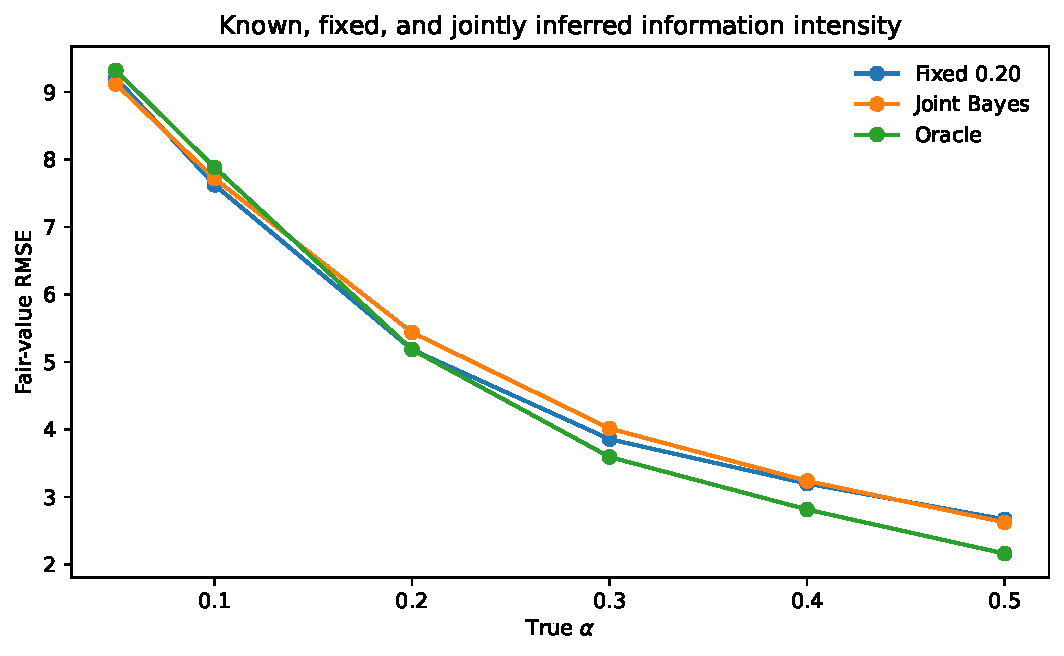
\includegraphics[width=0.80\textwidth]{08_unknown_alpha_rmse.pdf}
\caption{Fair-value RMSE when $\alpha$ is known, fixed, or jointly inferred.}
\label{fig:unknown-alpha}
\end{figure}

The joint estimator's mean terminal absolute error in $\alpha$ is \JointAlphaMae.

\begin{figure}[H]
\centering
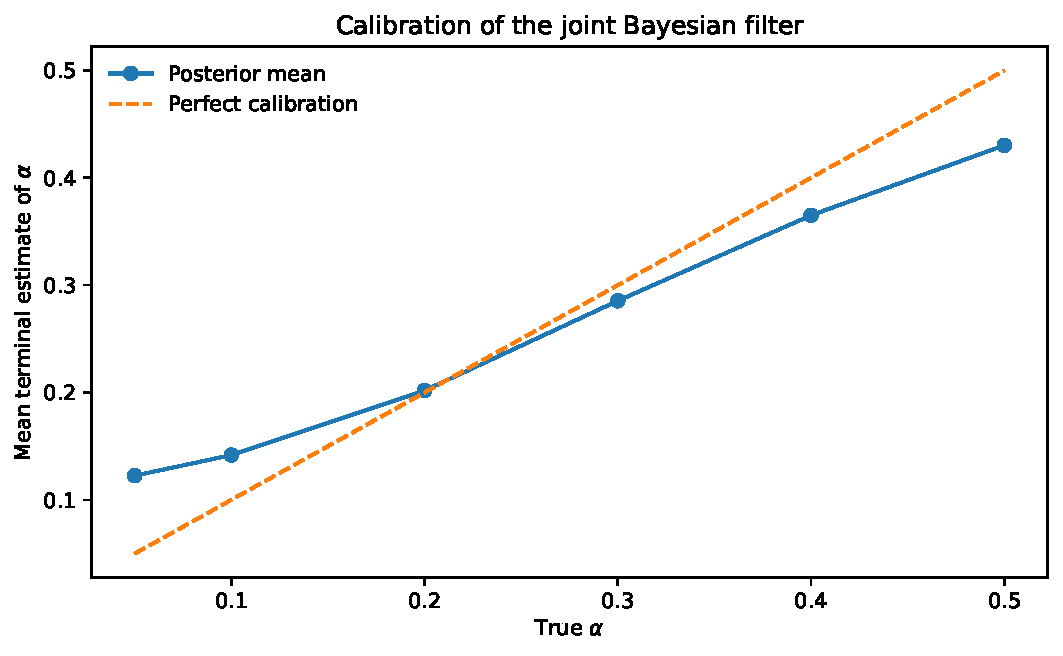
\includegraphics[width=0.80\textwidth]{09_alpha_calibration.pdf}
\caption{Calibration of the joint posterior mean for $\alpha$.}
\label{fig:alpha-calibration}
\end{figure}

The joint filter does not dominate the fixed rule in every short-horizon RMSE comparison. The reason is structural rather than computational. One observed order imbalance must carry information about both the sign of the hidden state and the strength of the signal process.

\subsection{Regime change}

The true informed-trader probability rises from $0.05$ to $0.40$ after 100 trades. Figure~\ref{fig:regime-alpha} compares a full-history joint filter with rolling windows.

\begin{figure}[H]
\centering
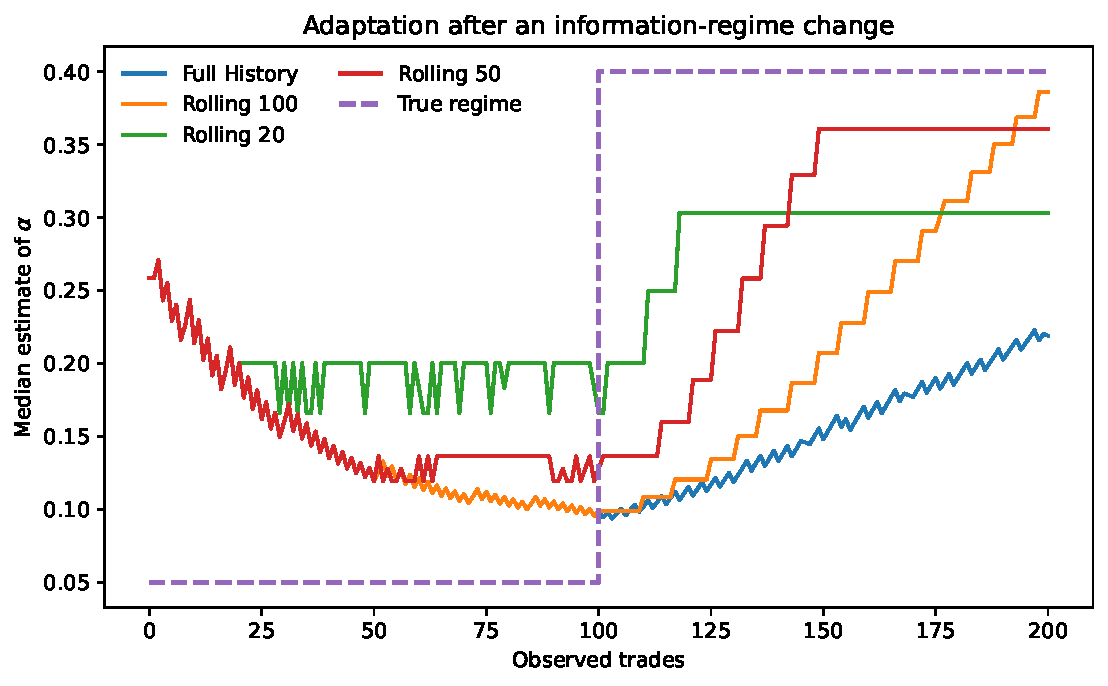
\includegraphics[width=0.86\textwidth]{10_regime_alpha_estimate.pdf}
\caption{Median estimate of $\alpha$ following a low-to-high information-regime change.}
\label{fig:regime-alpha}
\end{figure}

The 20-trade window reaches the stability criterion on \RollingReachRate\ of paths and, conditional on reaching it, has a median delay of \RollingMedianDelay\ trades. Its mean post-switch absolute error is \RollingPostMae. The full-history filter reaches the same criterion on only \FullHistoryReachRate\ of paths and has post-switch error \FullHistoryPostMae.

\begin{table}[H]
\centering
\caption{Adaptation after the regime change. Delay is reported only for paths satisfying the five-observation stability rule.}
\label{tab:regime}
\begin{tabular}{lccc}
\toprule
Estimator & Reach rate & Median delay & Post-switch MAE \\
\midrule
\RegimeRows
\bottomrule
\end{tabular}
\end{table}

\begin{figure}[H]
\centering
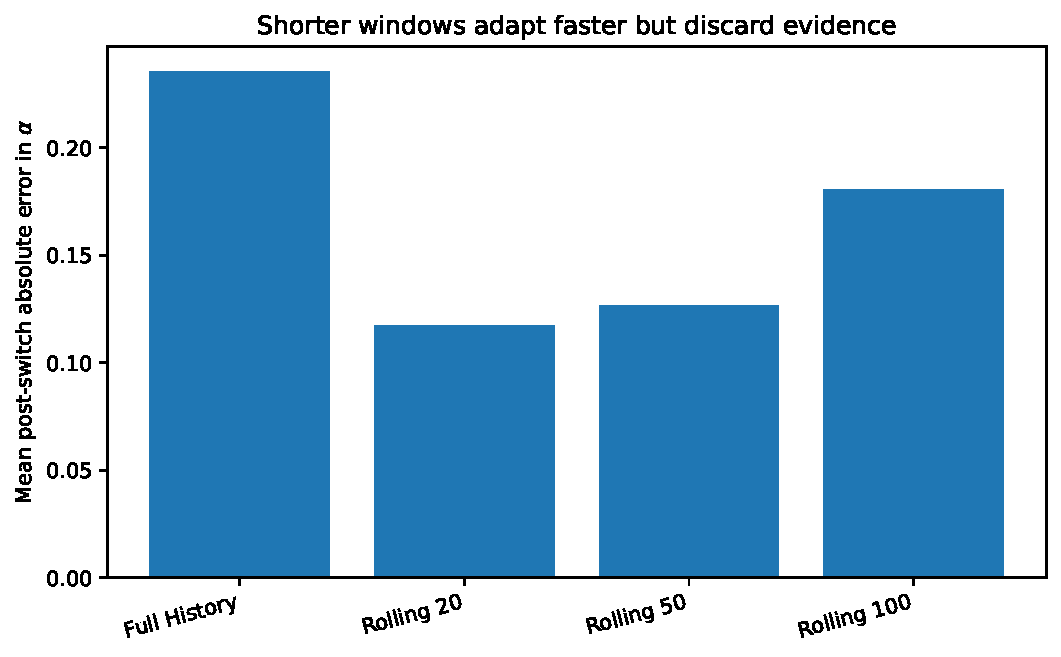
\includegraphics[width=0.78\textwidth]{11_regime_post_switch_error.pdf}
\caption{Mean post-switch error across full-history and rolling estimators.}
\label{fig:regime-error}
\end{figure}

Short memory adapts because old observations leave the sample. The same forgetting increases sampling variability. The 20-trade window performs well for this particular jump, horizon, grid, and tolerance; it is not a generally optimal regime filter.

\section{Discussion}

The analytical and numerical results support a narrow set of claims. Order direction is sufficient to create adverse-selection spreads and sequential learning in the binary model. The general-prior spread shrinks as posterior uncertainty disappears. A larger informed fraction widens the initial spread and increases the expected log-likelihood drift, so information risk and price discovery accelerate together.

Correctly specified competitive Bayesian quotes have zero conditional expected trade P\&L by construction. Their value in this model is better state inference and a different risk distribution, not positive expected profit. The static baseline is useful as a deliberately information-ignoring comparator, but its RMSE of 10 is mechanically implied by the symmetric binary setup.

Misspecification is more informative. Underestimating $\alpha$ creates a clear adverse-selection loss because the dealer treats informative flow as if it were closer to random. Overestimating $\alpha$ exposes the opposite problem: the exogenous execution model can reward implausibly wide quotes because customers never leave. That result is best treated as a failure mode of the simulator.

Joint inference introduces a genuine confounding problem between hidden value and information intensity. The regime experiment then shows the cost of a wrong stationarity assumption. A full-history posterior can be internally coherent while becoming a poor adaptive estimator after the data-generating process changes.

\section{Limitations}

The main limitations are structural:
\begin{enumerate}
\item The terminal value is binary and fixed throughout each information episode.
\item Informed traders know the terminal state perfectly and trade one unit without strategic timing or order splitting.
\item Noise traders buy and sell independently with equal probability.
\item The baseline information model has exogenous execution. Quote width does not affect participation.
\item There is one market maker, no price competition, queue position, latency, fees, rebates, tick size, partial fills, venue choice, or cross-asset hedge.
\item The joint-$\alpha$ model assumes the correct likelihood family and a small discrete parameter grid.
\item Value and information intensity are only weakly identified from one short order tape with one hidden terminal state.
\item The regime experiment contains one deterministic low-to-high jump. The rolling estimator is a heuristic rather than a latent-regime model.
\item The inventory appendix uses a Gaussian random walk and an imposed exponential fill curve. Neither is calibrated to market data.
\item The inventory simulator samples one customer side per step and caps fill probability at its base rate when inventory skew brings a quote to or through the public mid. Those choices affect its risk-return surface.
\item Information risk and inventory risk are not solved in a single equilibrium.
\item The checked-in outputs correspond to one principal seed profile. Common random numbers improve comparisons but do not establish robustness to alternative model families.
\item All outputs are simulated and do not constitute evidence of live-market profitability.
\end{enumerate}

These restrictions determine the range of valid interpretation. The project can test whether code, equations, accounting, and qualitative mechanisms agree under explicit assumptions. It cannot infer how a production market maker should quote a real instrument.

\section{Reproducibility and Software Design}

The primary simulator is written in OCaml and built with Dune. Hidden state is generated by the order-tape module and is never passed to the strategy interface. Quotes are computed before the current order side is observed. Strategies are evaluated on shared tapes, and each experiment accepts an explicit seed.

The numerical values in this document correspond to the \ResultsProfile\ run recorded in the manifest, using seed \ResultsSeed\ and engine \texttt{\ResultsEngine}. A separate Python implementation repeats the model equations without wrapping the OCaml executable. Its purpose is to expose disagreements in conditioning, signs, posterior timing, and aggregation.

The repository's continuous-integration workflow builds the OCaml source, runs the test suite, executes the reduced experiment profile, validates generated CSV files, rebuilds figures and LaTeX fragments, and compiles the report. The full-reproduction workflow runs the complete workload and records checksums.

One numerical implementation detail matters for robustness. Count-form joint likelihoods should be evaluated in log space rather than by directly multiplying thousands of probabilities. The revised implementation uses a log-sum-exp normalisation so valid long samples do not collapse to zero evidence through floating-point underflow.

\section{Conclusion}

The binary model is too small to resemble a real exchange. Its value is that mistakes are difficult to hide. Competitive quotes can be derived, posterior dynamics can be written as a random walk in log odds, expected information flow can be quantified, and P\&L can be reconciled in two independent ways.

The simulations are most useful when they fail gracefully. Underestimated information intensity generates adverse-selection losses for a clear reason. Overestimated information intensity reveals an execution artefact. Joint inference exposes weak identification. Regime change exposes a wrong stationarity assumption. The inventory appendix shows why a claim about quote placement requires a model in which price can affect whether an order trades.

The broader methodological lesson is simple: derive what can be derived, use those identities as test oracles, preserve the timing of information, compare strategies on the same random worlds, and treat attractive outputs as reasons to inspect assumptions before treating them as results.

\appendix
\section{Quote-Sensitive Inventory Stress Test}

The information model executes one trade at every step. It therefore cannot support a causal claim that widening or skewing quotes changes volume. A second environment introduces a public midprice
\begin{equation}
S_{t+1}=S_t+\sigma Z_t, \qquad Z_t\sim\mathcal{N}(0,1),
\end{equation}
and shifts the quote centre with inventory:
\begin{equation}
r_t=S_t-\beta q_t.
\end{equation}
The bid and ask are
\begin{equation}
B_t=r_t-\delta, \qquad A_t=r_t+\delta,
\end{equation}
and fill probability declines with quote distance:
\begin{equation}
P(Fill\mid d)=A_0e^{-kd}.
\end{equation}
This is a policy experiment, not an optimal-control derivation.

Moving the skew coefficient from $\beta=0$ to $\beta=0.10$ reduces mean maximum absolute inventory by \InventoryExposureDrop\ and P\&L standard deviation by \InventoryRiskDrop. Mean P\&L falls by \InventoryMeanPnlDrop\ over the same comparison.

\begin{figure}[H]
\centering
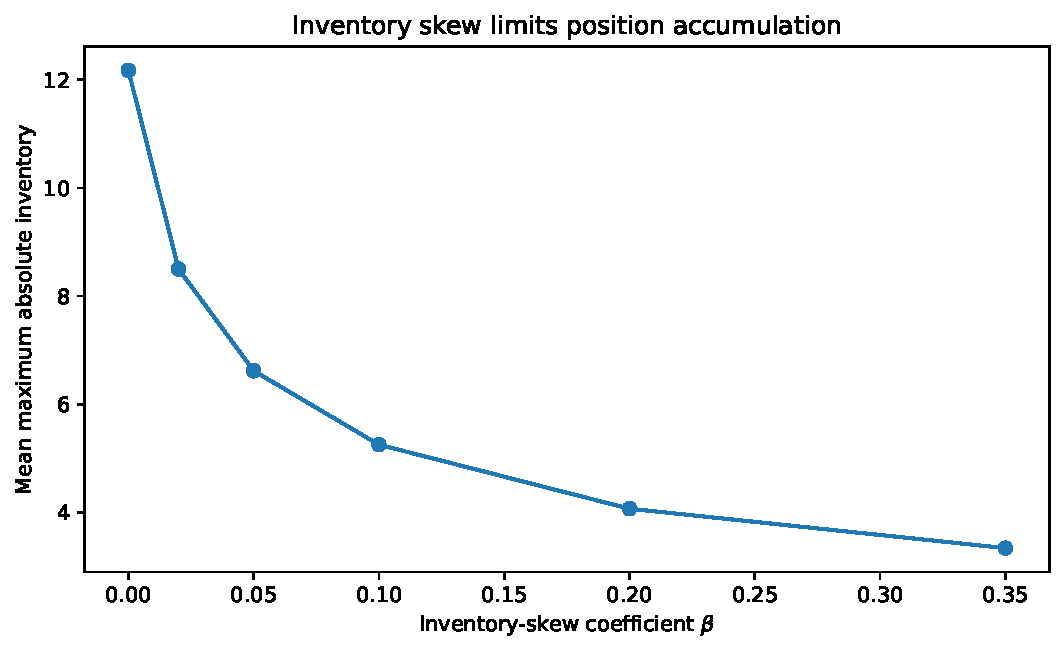
\includegraphics[width=0.78\textwidth]{12_inventory_exposure.pdf}
\caption{Inventory exposure as the quote centre becomes more inventory-sensitive.}
\label{fig:inventory-exposure}
\end{figure}

\begin{figure}[H]
\centering
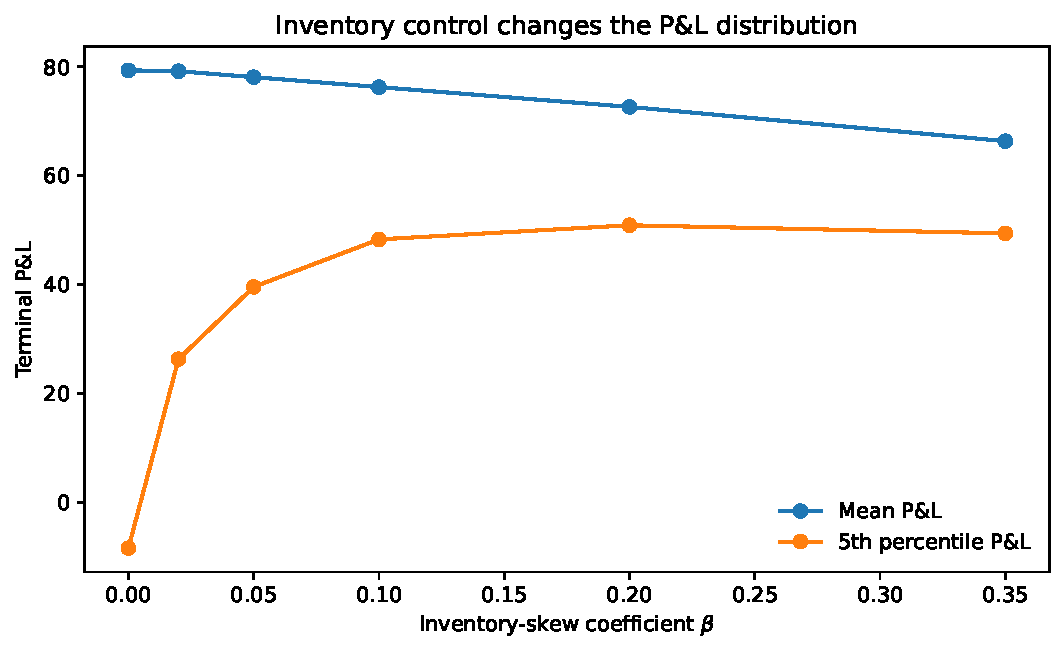
\includegraphics[width=0.78\textwidth]{13_inventory_pnl.pdf}
\caption{Mean and fifth-percentile P\&L under inventory skew.}
\label{fig:inventory-pnl}
\end{figure}

Once fills depend on quote distance, a wider market is no longer mechanically better. Mean P\&L peaks at a half-spread of \BestHalfSpread, where the model produces approximately \BestHalfSpreadPnl\ units of terminal P\&L and \BestHalfSpreadFills\ fills per episode.

\begin{figure}[H]
\centering
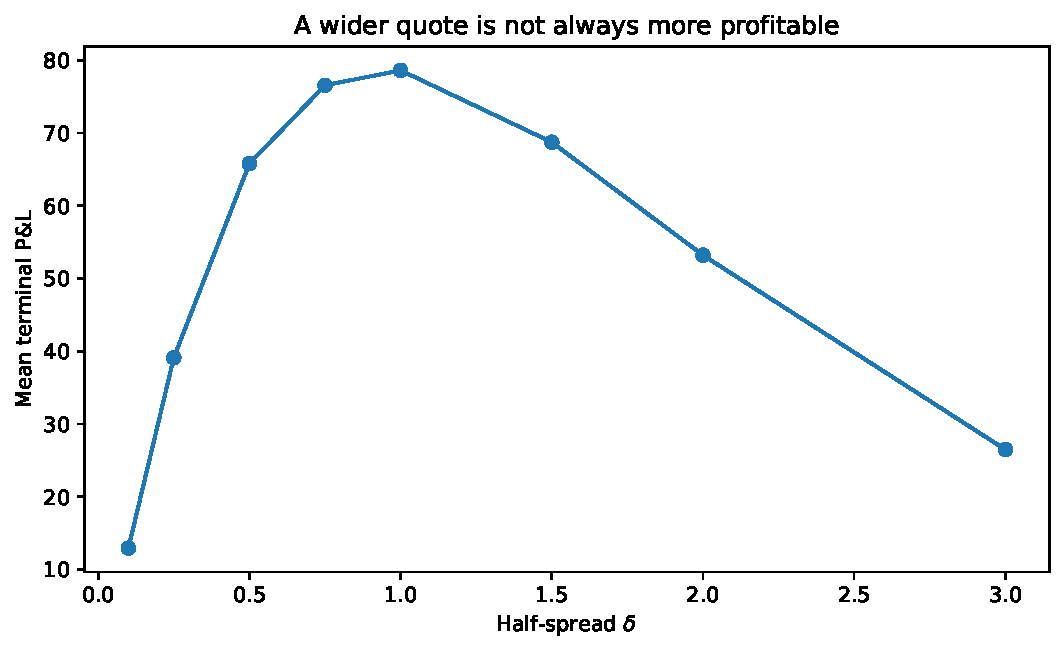
\includegraphics[width=0.78\textwidth]{14_quote_distance_pnl.pdf}
\caption{Mean P\&L as quote distance changes.}
\label{fig:quote-pnl}
\end{figure}

\begin{figure}[H]
\centering
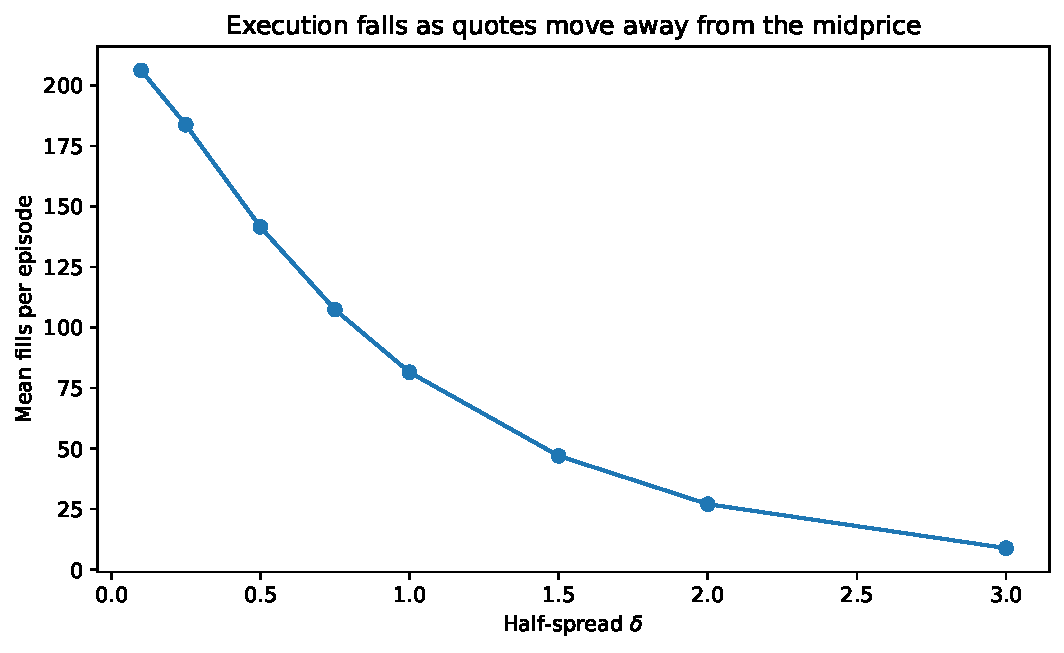
\includegraphics[width=0.78\textwidth]{15_quote_distance_fills.pdf}
\caption{Execution count as quote distance changes.}
\label{fig:quote-fills}
\end{figure}

The interior maximum is a property of the imposed fill curve, volatility, horizon, and parameter grid. It is not an estimate of a real-market optimal spread.

\begin{thebibliography}{9}

\bibitem{glosten_milgrom_1985}
Lawrence R. Glosten and Paul R. Milgrom.
\newblock Bid, Ask and Transaction Prices in a Specialist Market with Heterogeneously Informed Traders.
\newblock \emph{Journal of Financial Economics}, 14(1):71-100, 1985.
\newblock \url{https://doi.org/10.1016/0304-405X(85)90044-3}.

\bibitem{das_2005}
Sanmay Das.
\newblock A Learning Market-Maker in the Glosten-Milgrom Model.
\newblock \emph{Quantitative Finance}, 5(2):169-180, 2005.
\newblock \url{https://doi.org/10.1080/14697680500148067}.

\bibitem{ohara_1995}
Maureen O'Hara.
\newblock \emph{Market Microstructure Theory}.
\newblock Blackwell, 1995.

\bibitem{avellaneda_stoikov_2008}
Marco Avellaneda and Sasha Stoikov.
\newblock High-Frequency Trading in a Limit Order Book.
\newblock \emph{Quantitative Finance}, 8(3):217-224, 2008.
\newblock \url{https://doi.org/10.1080/14697680701381228}.

\bibitem{gueant_2013}
Olivier Gu\'eant, Charles-Albert Lehalle, and Joaquin Fernandez-Tapia.
\newblock Dealing with the Inventory Risk: A Solution to the Market Making Problem.
\newblock \emph{Mathematics and Financial Economics}, 7(4):477-507, 2013.
\newblock \url{https://doi.org/10.1007/s11579-012-0087-0}.

\bibitem{adams_mackay_2007}
Ryan Prescott Adams and David J. C. MacKay.
\newblock Bayesian Online Changepoint Detection.
\newblock arXiv:0710.3742, 2007.
\newblock \url{https://doi.org/10.48550/arXiv.0710.3742}.

\end{thebibliography}

\end{document}
